\documentclass{llncs}
\usepackage{geometry}
\geometry{
  a4paper,         % or letterpaper
  textwidth=16cm,  % llncs has 12.2cm
  textheight=24cm, % llncs has 19.3cm
  heightrounded,   % integer number of lines
  hratio=1:1,      % horizontally centered
  vratio=2:3,      % not vertically centered
}

\renewcommand\labelitemi{*}

% Packages
% ------------------
\usepackage{bm} % bold mode
\usepackage{subfig}
\usepackage{graphicx}
\usepackage{hyperref}
\usepackage{amssymb}
\usepackage{amsmath}
\usepackage{color}
\usepackage{dsfont}

%% new commands
% ------------------
\definecolor{light-gray}{gray}{0.95}
\newcommand{\code}[1]{\colorbox{light-gray}{\texttt{#1}}}


\begin{document}


% % Bibliography variables
% % -----------------------
% \bibliographystyle{ieeetr}


% Header of paper
% ---------------------
\title{WCAG Compliance Guide for \LaTeX Docs }

\author{Sergio Garc\'{i}a-Vergara}

\institute{\email{sergiodotgarcia@gmail.com}}

\maketitle


%@@@@@@@@@@@@@@@@@@@@@@@@@@@@@@@@@@@@@@@@@@@@@@@@@@


% Abstract
% ---------------------
\begin{abstract}
  This document details the steps for generating \LaTeX documents to be WCAG
  compliant. The goal is for screenreaders to accurately handle the compiled
  documents. Namely, this means reading the document in order, and handling the
  math equations and section headings accurately.

% \begin{keywords}
%   one $\cdot$ two
% \end{keywords}

\end{abstract}


% @@@@@@@@@@@@@@@@@@@@@@@@@@@@@@@@@@@@@@@@@@@@@@@@@@

\section{Introduction}
% ---------------------------

Web Content Accessibility Guidelines (WCAG) are a set of recommendations for
making Web content more accessible. For a document to be considered to be WCAG
compliant, the following need

\begin{itemize}
\item \textbf{Use semantic markup}: Make sure to use semantic markup in your
  \LaTeX document. This means using the appropriate \LaTeX commands for
  headings, lists, tables, and other elements. This will help screen readers and
  other assistive technologies to understand the structure of the document.

\item \textbf{Provide alternative text for images}: Use the
  \textit{includegraphics} command to include images in your \LaTeX document,
  and provide alternative text for each image using the alt parameter. The
  alternative text should describe the content or function of the image.

\item \textbf{Use accessible colors}: Choose colors that have sufficient
  contrast for people with color vision deficiencies. You can use online tools
  such as the WebAIM Contrast Checker to check the contrast ratio of your color
  combinations.

\item \textbf{Use appropriate font sizes}: Use a minimum font size of 12pt for
  body text, and larger sizes for headings and other important elements. This
  will ensure that the text is legible for all users.

\item \textbf{Add metadata}: Add metadata to your document, including title,
  author, and language information. You can do this using the hyperref package
  in \LaTeX.

% \item Add tags to the PDF: Finally, you can add tags to your PDF document using
%   the tagpdf package in \LaTeX. This will provide a structured representation of
%   the document for assistive technologies.

\end{itemize}


This guide describes the steps that authors should follow to generate accessible
documents using \LaTeX. Namely, this guide will walk you through correctly
handling:

\begin{itemize}
  \item section and subsection headers
  \item embedded URLs
  \item math equations
  \item figures and images
  \item tables
\end{itemize}



\subsection{tex4t: Command-line Tool}
% ---------------------------

Overall, while PDF documents can be made WCAG compliant, HTML is often a more
accessible format for online content. By using the \code{tex4ht} package to
convert your \LaTeX document to HTML, you can make your content more accessible
to a wider audience.

% ==================================================
% TODO: write a few sentences about the tex4ht package
% ==================================================

% @@@@@@@@@@@@@@@@@@@@@@@@@@@@@@@@@@@@@@@@@@@@@@@@@@

\section{Document-level Instructions}
% ---------------------------

The following sections describe what authors need to do in their \textit{.tex}
files such that documents are WCAG compliant. The instructions for generating
the appropriate HTML files (once the \textit{.tex} file is complete), are
described in Section \ref{sec:Compiling .tex file to HTML}: \textit{Compiling
  .tex file to HTML}.


\subsection{Images and Figures}
% ---------------------------

Figure and images included in your document need to be accompanied by
alternative text.

The following is an example:

\begin{figure}
  \centering
  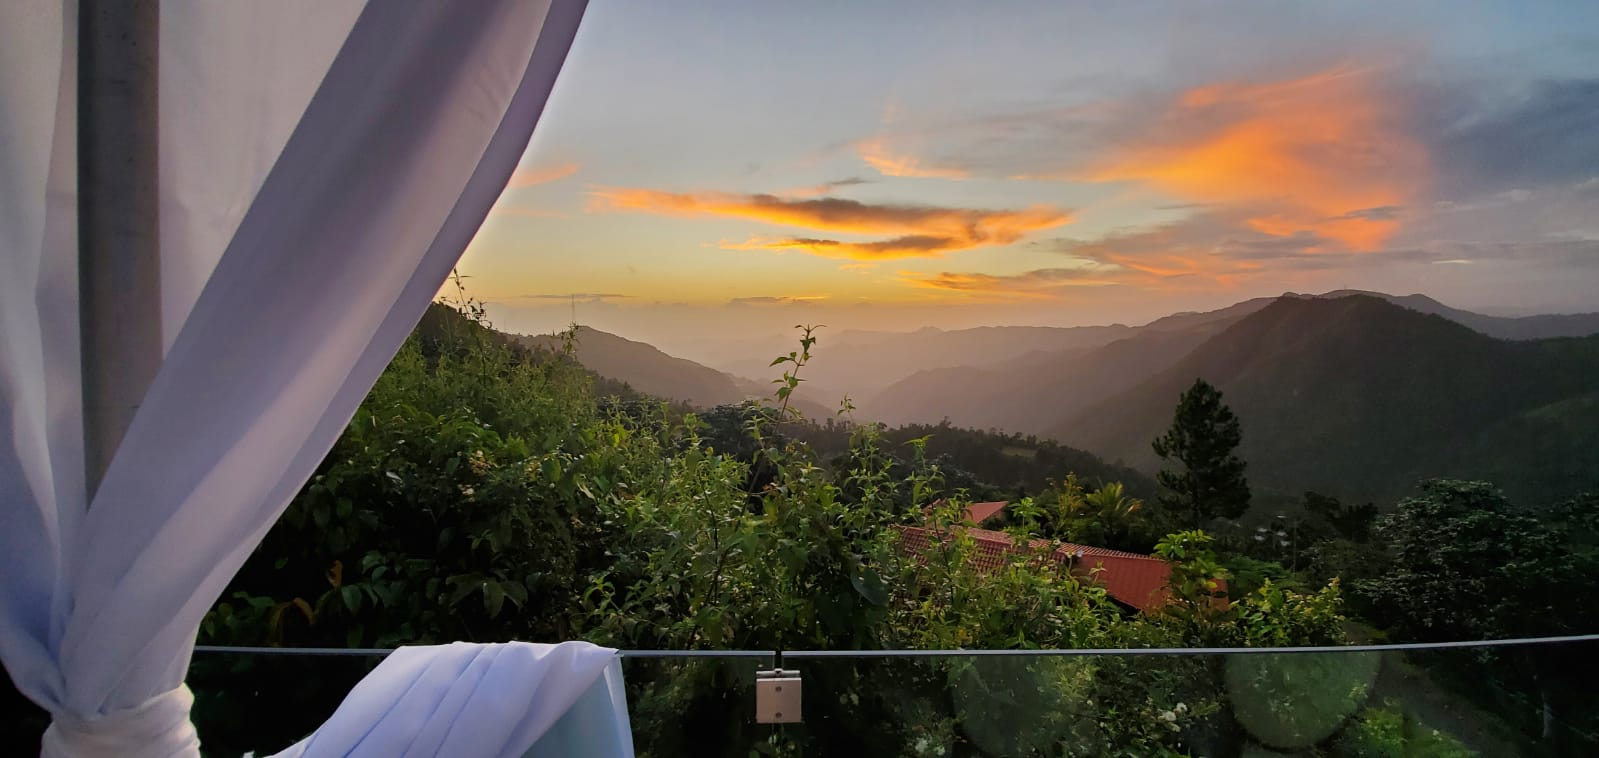
\includegraphics[alt={Alt Text}, width=10cm]{figs/Cayey.jpeg}
  % 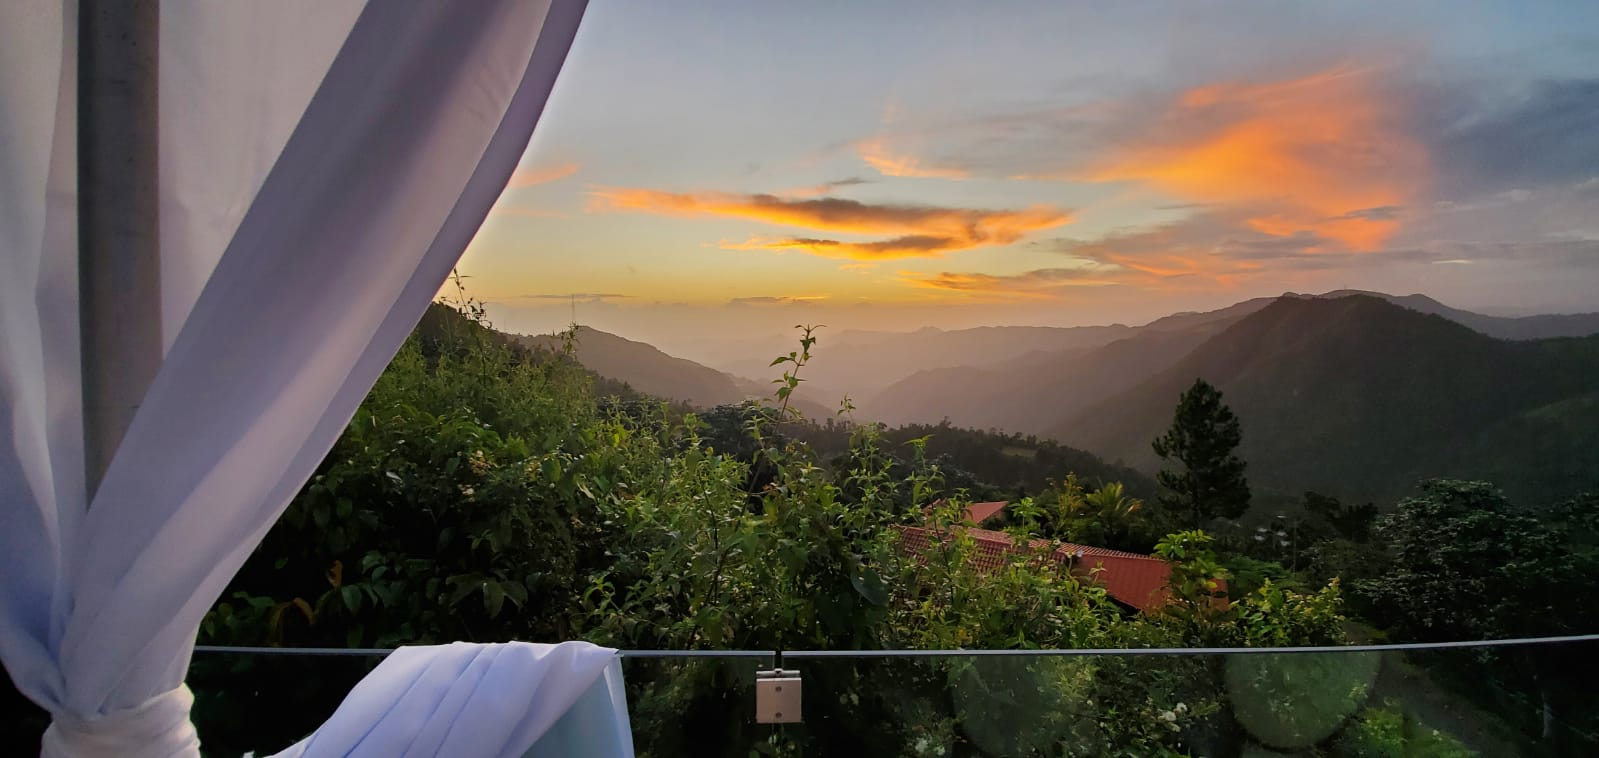
\includegraphics[width=10cm]{figs/Cayey.jpeg}
  \caption{Cayey, PR}
  \label{fig:earth}
\end{figure}


\subsection{Equations}
% ---------------------------

The following is a math equation:

\begin{equation}
  y = \frac{1 + \sqrt{5}}{2}
\end{equation}


% @@@@@@@@@@@@@@@@@@@@@@@@@@@@@@@@@@@@@@@@@@@@@@@@@@

\section{Compiling .tex file to HTML}
\label{sec:Compiling .tex file to HTML}
% ---------------------------

\subsection{Ubuntu}
% ---------------------------


\subsection{Widows}
% ---------------------------


% @@@@@@@@@@@@@@@@@@@@@@@@@@@@@@@@@@@@@@@@@@@@@@@@@@

\section{Other Methods}
% ---------------------------

As I worked on putting together this guide, I found several tools for
automatically tagging PDFs


% @@@@@@@@@@@@@@@@@@@@@@@@@@@@@@@@@@@@@@@@@@@@@@@@@@



% -----------------------------
%% \bibliography{references}


% -----------------------------
\end{document}

%%% Local Variables:
%%% mode: latex
%%% TeX-master: t
%%% End:
